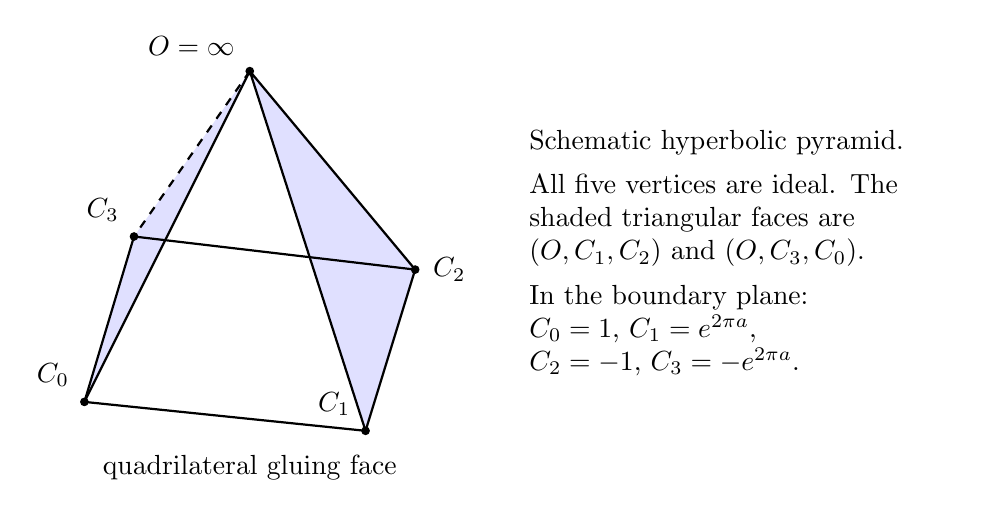
\begin{tikzpicture}[scale=1.05]
\coordinate (c0) at (-2,-1);\coordinate(c1) at (1.4,-1.35);\coordinate(c2) at (2,.6);\coordinate(c3) at (-1.4,1);\coordinate(o) at (0,3);
\fill[blue!12] (o)--(c1)--(c2)--cycle;\fill[blue!12] (o)--(c3)--(c0)--cycle;
\draw[thick] (c0)--(c1)--(c2)--(c3)--cycle;
\draw[thick] (o)--(c0) (o)--(c1) (o)--(c2);\draw[thick,dashed] (o)--(c3);
\foreach \p/\l in {c0/C_0,c1/C_1,c3/C_3,o/O=\infty}{\fill (\p) circle(1.5pt);\node[above left=2pt] at (\p) {$\l$};}
\fill (c2) circle(1.5pt);\node[right=3pt] at (c2) {$C_2$};
\node at (0,-1.8) {quadrilateral gluing face};
\node[align=left,text width=5.5cm] at (6,.8) {Schematic hyperbolic pyramid.\\[4pt]All five vertices are ideal. The shaded triangular faces are $(O,C_1,C_2)$ and $(O,C_3,C_0)$.\\[4pt]In the boundary plane:\\ $C_0=1$, $C_1=e^{2\pi\ii a}$,\\ $C_2=-1$, $C_3=-e^{2\pi\ii a}$.};
\end{tikzpicture}
